%
\documentclass[parskip,headsepline, headtopline, %
footsepline, oneside, 12pt, headings=small]{scrreprt}
\usepackage[ngerman]{babel}
\usepackage[utf8]{inputenc}
\usepackage{color}
\usepackage{pdfpages} % To include other PDFs
\usepackage{changepage} 
\usepackage{textcomp}
% To insert dummy text
\usepackage{blindtext}
\setcounter{secnumdepth}{2}
 
% Provide a command to include pretty quotes
\usepackage{ragged2e} %justify dictum
\renewcommand*{\dictumwidth}{.5\textwidth}
\newcommand{\setChapterQuote}[3]{\setchapterpreamble[o]{%
\dictum[#2 \emph{#3}]{\justifying {#1}}}}
 
%Set font to times
\usepackage{txfonts}
 
% Define own Chapter style
% Pretty chapter pages
%------------------------------------------
\definecolor{nicered}{rgb}{.647,.129,.149}
\usepackage{soul}

% hyperref has to be used last
\usepackage{hyperref}
\makeatletter
\newsavebox{\feline@chapter}
\newcommand\feline@chapter@marker[1][4cm]{%
\sbox\feline@chapter{%
\resizebox{!}{#1}{\fboxsep=1pt%
\colorbox{grey}{\color{white}\bfseries\sffamily\thechapter}%
}}%
\rotatebox{90}{%
\resizebox{%
\heightof{\usebox{\feline@chapter}}+\depthof{\usebox{\feline@chapter}}}%
{!}{\scshape\so\@chapapp}}\quad%
\raisebox{\depthof{\usebox{\feline@chapter}}}{\usebox{\feline@chapter}}%
}
\newcommand\feline@chm[1][4cm]{%
\sbox\feline@chapter{\feline@chapter@marker[#1]}%
\makebox[0pt][l]{% aka \rlap
\makebox[1cm][r]{\usebox\feline@chapter}%
}}   
 
\renewcommand*{\chapterformat}{%
\hspace{\leftmargin} \feline@chm[2.5cm] % Height of the colored box
\hspace{2cm}
}
\makeatother
%------------------------------------------
% ------------------------------------------------------------------------------
\newcommand{\HRule}[1]{\hfill \rule{0.2\linewidth}{#1}}         % Horizontal rule

\definecolor{grey}{rgb}{0.9,0.9,0.9} 

\makeatletter                                                   % Title
\def\printtitle{%                                               
    {\centering \@title\par}}
\makeatother                                                                    

\makeatletter                                                   % Author
\def\printauthor{%                                      
    {\centering \large \@author}}                               
\makeatother                                                    

% ------------------------------------------------------------------------------
% Metadata (Change this)
% ------------------------------------------------------------------------------
\title{ \fontsize{50}{60}\selectfont \vspace{2.10cm}
\hfill \begin{huge}{\fontfamily{@arialn}\selectfont {\fontfamily{txtt}\selectfont The Design for All}}\end{huge}
 \hfill \large{\begin{flushright}Psychologie, Design, Emotionen\end{flushright}} \vspace{1.9cm}
 \hfill \small{Design for All \textbackslash\textbackslash Susanne Maaß \textbackslash\textbackslash  Wintersemester 2012/2013 \textbackslash\textbackslash  \today} 
}
\author{
                \hfill Martha Rohte (2259987) und Maria Meister (2142018)\\  
                \hfill Universität Bremen\\   
                \hfill Fachbereich Mathematik \& Informatik \\
        \hfill \texttt{\fontfamily{cmr}\selectfont mata@informatik.uni-bremen.de} \\
        \hfill \texttt{\fontfamily{cmr}\selectfont mmeister@informatik.uni-bremen.de} \\
}


\renewcommand{\sfdefault}{@sshlined}
\begin{document}

% ------------------------------------------------------------------------------
% Maketitle
% ------------------------------------------------------------------------------
\thispagestyle{empty}                           % Remove page numbering on this page



\colorbox{grey}{
        \parbox[t]{1.14\linewidth}{
                \printtitle 
                \vspace*{0.2cm}               
        }
}
        \vfill
\printauthor                                                            % Print the author data as defined above
\HRule{1pt}

\clearpage

%\begin{abstract}

%\end{abstract}
% NOTE: '?' is placeholder for selected text 
% or caret location (when no selection).

%Die Ausarbeitung sollte mindestens folgende Teile haben
%• Titelblatt mit Angaben zum Thema, VerfasserInnen mit Matrikelnummern,
%Veranstalterin, Veranstaltung, Semester, Datum...
%• Gliederung/ Inhaltsverzeichnis
%• eine Einleitung, die auch die Struktur des Papiers beschreibt,
%• formulierte Übergänge zwischen den Abschnitten,
%• eine Zusammenfassung am Schluss und
%• ein vollständiges Verzeichnis der verwendeten Literatur/Quellen
%• Seitenzahlen!
%Umfang: pro Person in der Vorbereitungsgruppe erwarte ich 8-10 Seiten.
%Schriftgröße Arial 11 oder Times New Roman 12. Seitenränder 2,5 cm

\tableofcontents
 
% Chapter 0

\section{Einleitung}


% Chapter A
\setChapterQuote{A thought is an idea in transit.}{Pythagoras}{582 B.C. - 497 B.C.}
\chapter{Alltagsdesign}


Der das Buch geschrieben hat, ursprünglich Psychologe, setzt er sich immer mehr mit der Benutzbarkeit zuerst von Alltagsgegenständen und auch von informatischen Produkten auseinander. Sein Buch \glqq Psychology of Everyday Things \grqq ist zu großer Beliebtheit in den Kreisen der Usability Forschung und des Designs gelangt. 


Norman sieht den Ursprung von schlechten Design hauptsächlich in einen Phänomen, welches er in seinem Buch als Technologieparadoxon wie folgt beschreibt \cite[S.31]{don}:\\

\glqq Whenever the number of functions and required operations exceeds the number of controls, the design becomes arbitrary, unnatural, and complicated. 
	The same technology that simplifies life by providing more functions in each device also complicates life by making the device harder to learn, harder to use. This is the paradox of technology.\grqq 

Oder anders ausgedrückt Systeme werden immer komplexer, da sie über im mehr Funktionalitäten verfügen, allerdings können diese aufgrund ihrer Anzahl nicht eindeutig abgebildet werden, was dazu führt das Funktionen oft nur durch Kombination anderer Funktionen ausgeführt werden können. Durch Umstand erhöht sich die Komplexität von Systemen immens. Zusätzlich dazu bekommt der Benutzer meist nur wenig Feedback, ob seine Interaktion mit dem System erfolgreich war. darauf wird gerne zu Gunsten des Designs verzichtet. 


\section{Designaspekte}
\label{sec:aspekte}

Laut Norman ist das zentrale Prinzip von Designen, Dinge so zu entwerfen, dass die Erwartungshaltung des Nutzers bezogen auf die Funktionsweise der einzelnen Elemente auch mit ihrer tatsächlichen Funktionalität übereinstimmt, sodass der Nutzer in der Lage versetzt wird akkurat agieren zu können.\\ 
Als Ausgangsbedingung dafür gibt es fünf zentrale Aspekte, die eingehalten werden müssen, um  ein möglichst intuitives Design bereitzustellen. Die Prinzipien 
	
Unter den Aspekt der \textbf{Sichtbarkeit} versteht Norman Funktionalitäten transparent zu gestalten. Beispielsweise muss bei öffentlichen Waschbecken ersichtlich gemacht werden, ob diese manuell durch Knöpfe oder über Sensoren reguliert werden.\\
   
Des Weiteren ist ein unabgegänlicher Aspekt, der des \textbf{Feedback}s. Darunter versteht man jegliche Rückmeldung des Systems, über Auswirkungen von Aktionen, sowie der daraus folgende interne Zustand des Systems. Das Feedback kann auf visueller (z.B Signalleuchten) oder auch auf akustischer Ebene erfolgen.\\
 
Das	\textbf{Mapping} bezieht sich darauf die inhärenten Funktionen des Systems auf einer Art und Weise abzubilden, sodass sie nicht nur eindeutig identifizierbar sind, sondern auch intuitiv verständlich.\\

Der Aspekt der \textbf{Affordanz} basiert auf den Affordanzbegriff, der 1977 im Artikel 'The Theory of Affordances' von James Jerome Gibson eingeführt wurde. Der Begriff Affordanz leitet sich vom Englischen “to afford”(“leisten”, “anbieten”, “gewähren”) ab. Laut Gibson leiten sich Affordanzen aus Komplementarität von Umwelt und Lebewesen ab, d.h.  
die Handlungsanregung von Dinge aufgrund der Informationen über ihre funktionell relevante Eigenschaften oder Bestandteilen der Umwelt. Dieses Zusammenspiel ermöglicht oder viel mehr suggeriert ein bestimmtes Verhalten. Wodurch die Affordanz maßgeblich für Funktionalität und Intuitivität eines Gegenstandes wird.
Norman erweiterte diese Defintionsbegriff um den der \textit{wahrgenomme} Affordanz. Darunter fallen auch suggerierte Affordanzen, die gar nicht tatsächlich bestehen, wie beispielsweise aufgemalte Türen durch die man nicht gehen kann oder der Computermonitor, der trotz seiner Begebenheiten nicht haptisch benutzbar ist. 

\begin{figure}
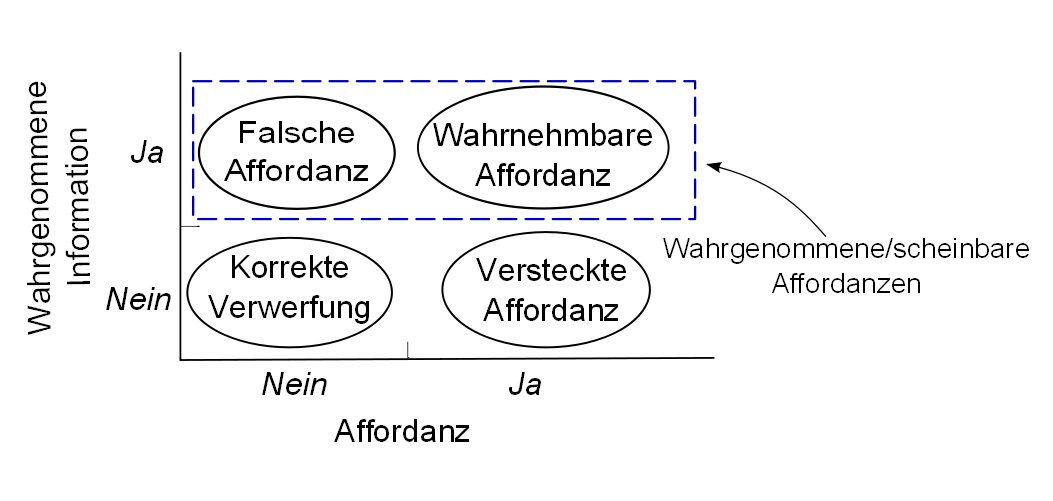
\includegraphics{images/figure2_affordances.png}
\caption{Affordanzen}
\label{fig:action}
\end{figure}

Der Designaspekt Contraints beschreibt Beschränkungen, die aufgrund bestimmmter Begebenheiten entstehen. Die Begebenheiten können von \textit{physisch}, \textit{semantisch}, \textit{kulturell} oder \textit{logische} Art sein.

\section{Konzeptuelle Modelle}


\section{Aktion}

Nach Norman laufen die Aktionen in einem Zyklus ab (Vgl. Abb. \ref{fig:action}, \cite[S. 46ff]{don}). Dieser besteht aus zwei Teilen: dem Gulf of Execution und dem Gulf of Evaluation. Zuerst muss der Handelnde in seinem Kopf ein Ziel bilden wie zum Beispiel \glqq Ich möchte lesen (können, aber dazu ist es zu dunkel).\grqq Um eine Handlung auszuführen, muss er nun den Gulf of Execution überbrücken. Hierzu muss er zuerst die Intention bilden \glqq Ich schalte die Leselampe an.\grqq, die Aktion spezifizieren \glqq Ich muss den Arm ausstrecken, den Schalter fassen und den Schalter umlegen.\grqq und die Aktion schließlich auch wirklich ausführen. Als Resultat ändert sich der Zustand der Welt. Um diesen wahrzunehmen und zu bewerten, muss der Handende nun den Gulf of Evaluation überbrücken. Dies beginnt damit, dass der Zustand der Welt wahrgenommen wird \glqq Es ist (nicht) hell.\grqq Danach wird der Zustand der Welt interpretiert: \glqq Die Lampe scheint (nicht).\grqq Letztlich wird das Ergebnis evaluiert: \glqq Ich kann jetzt (immer noch nicht) lesen.\grqq

\begin{figure}
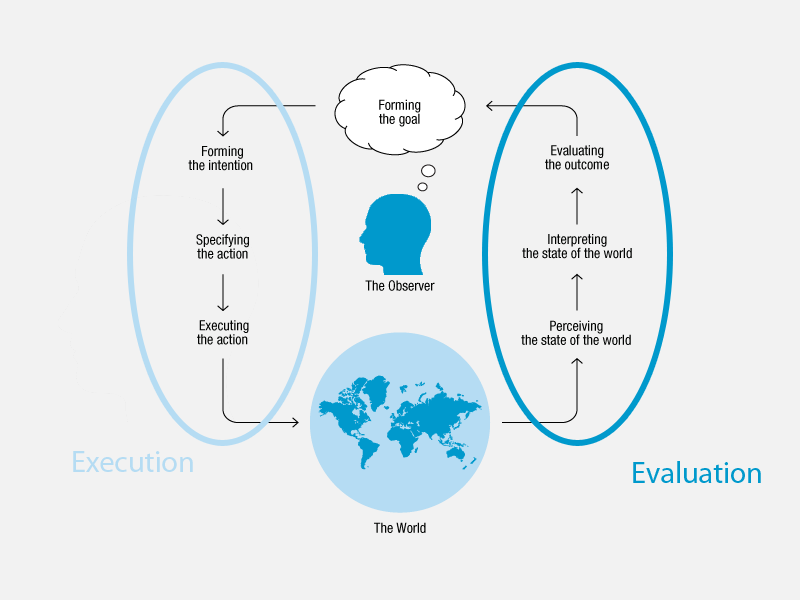
\includegraphics[width=\textwidth]{images/ActionCycle.png}
\caption{Der Aktionszyklus von Norman}
\label{fig:action}
\end{figure}

Damit ist dieser Zyklus beendet. Ist das Ergebnis positiv, so wird ein neuer Zyklus begonnen oder ein übergeordneter Zyklus fortgesetzt (\glqq Ich lese das Buch. / Ich fange an das Buch zu lesen. \grqq). Ist das Ergebnis hingegen negativ, so wird der Zyklus entweder mit einer anderen Intention wiederholt (\glqq Ich will Licht. \textrightarrow Ich schalte die Zimmerlampe an. \grqq) oder der Zyklus wird verfeinert (\glqq Ich überprüfe die Funktionsfähigkeit der Lampe: Hat sie Strom? Ist die Glühlampe defekt?  \grqq). Die verschiedenen Aktionszyklen können beliebig ineinander übergehen bzw. verschachtelt werden. 

Ein gutes Design verkleinert dabei die beiden Gulfs soweit wie möglich, denn je geringer die Schritte sind, desto unwahrscheinlicher ist es Fehler zu machen und umso weniger Zeit vergeht eine Aktion auszuführen. Für die Ausführung sind dabei die Sichtbarkeit, das Mapping, die Affordanzen und die Constraints entscheidend; all dies kann bei guter Anwendung die Überquerung des Gulf of Execution vereinfachen. Hingegen ist für die Evaluation das Feedback am wichtigsten, denn dieses wird an der Veränderung der Welt gemessen. Je direkter und einfacher zu interpretieren das Feedback ist, umso schmaler ist der Gulf of Evaluation. Ein gutes Beispiel hierfür sind die altbekannten Lampen: sobald man den Schalter gedrückt hat geht die Lampe an --- oder eben auch nicht. Wobei bei neueren Lampen, so wie zum Beispiel Energiesparlampen, das Feedback zwar noch ausreichend aber nicht mehr ganz so überragend ist: die Lampen leuchten oft nur verzögert auf oder werden erst kontinuierlich hell, im ersten Moment mag der uneingeweihte Benutzer vermuten, dass die Lampe defekt ist. 
%Bsp. einfaches aber aufwändigeres Feedback ist Flicken vom Fahrradschlauch: Ist er dicht?

\section{Fehler}

Da irren nun einmal menschlich ist, unterlaufen allen Menschen gelegentlich Fehler. Norman unterscheidet diese Fehler in zwei grundlegende Arten \cite[S. 105]{don}: Die Erste sind die Fehlleistungen, im Englischen \glqq Slips\grqq  genannt. Diese beschreiben unintendierte Handlungen. Die Zweite sind die Irrtümer, im Englischen \glqq Mistakes\grqq. Sie beschreiben nicht erwartete und erwünschte Ergebnisse, die auf vermeintlich korrekte Handlungen folgen.

\subsection{Fehlleistungen (Slips)}

Die Fehlleistungen beruhen im Allgemeinen darauf, dass eine Handlung automatisiert abläuft oder unaufmerksam auf Grund ihrer (vermeintlichen) Einfachheit ausgeführt wird. Sie sind meist einfach zu erkennen und sollten in einem guten Design einfach zu berichtigen sein.

Norman unterscheidet sechs verschiedene Arten von Fehlleistungen\cite[S. 107]{don}:

\begin{itemize}
\item \textbf{Fangfehler} sind Fehler, die passieren, wenn die Anfangssequenz von zwei Aktionen identisch sind, wobei die beabsichtigte Aktion unvertrauter ist und daher von der vertrauteren \glqq aufgefangen\grqq wird. Zum Beispiel, wenn man sein Geburtsdatum schreiben soll, aber als Jahr das aktuelle Jahr einträgt.
\item \textbf{Beschreibungsfehler} erfolgen, wenn zwei Aktionen viel Ähnlichkeit miteinander haben. Oft wird nur ein Gegenstand dabei ausgewechselt, also zum Beispiel wird die Dreckwäsche nicht in den Wäschekorb, sondern in die Toilette wirft, die direkt daneben steht: Aufklappen -- reinwerfen -- zuklappen.
\item \textbf{Datengesteuerte Fehler} kommen vor, wenn man zwei verschiedene Daten miteinander vertauscht, vor allem, wenn man das falsche Datum in dem Moment sieht, wenn man also zum Beispiel statt der Telefonnummer die Raumnummer wählt.
\item \textbf{Fehler durch assoziative Aktivierung} finden dann statt, wenn die Impulse zur Aktivierung dieser Aktionen ähnlich sind und deshalb die falsche Handlung ausgeführt wird, zum Beispiel, wenn man in das Telefon \glqq Herein!\grqq  ruft.
\item \textbf{Fehler durch Aktivierungsverlust} geschehen aufgrund einer Aktion, die während einer anderen Handlung ausgeführt wird, diese vergessen wird. Das typische Beispiel ist, dass man nachdem man die Tür zu einem Raum geöffnet hat und in diesem steht man nicht mehr weiß, was man dort tun wollte.
\item \textbf{Modus-Fehler} treten ausschließlich auf, wenn Geräte verschiedene Modi haben. Wird versucht eine Handlung auszuführen, die in einem Modus nicht möglich ist, obwohl sich das Gerät in diesem befindet, so ist dies ein Modus-Fehler. Ein Beispiel ist, wenn man versucht in einem Dokument zu schreiben während dieses im schreibgeschützten (read-only) Modus geöffnet ist.
\end{itemize}

Nach Möglichkeit sollte während des Designvorgangs darauf geachtet werden, dass diese Fehlleistungen vermieden werden, dass das Design also möglichst Fehlertolerant ist. Aus diesem Grund sind zum Beispiel in einem Firmennetzwerk häufig die Telefonnummern mit den Raumnummern identisch.

\subsection{Irrtümer (Mistakes)}

Irrtümer sind im Gegensatz zu Fehlleistungen oft nur schwer oder spät zu erkennen und deshalb auch nur schwer zu vermeiden. Hinzu kommt, dass sie oft weitaus drastischere Folgen als Fehlleistungen haben. Sie sind das Resultat von dem Verfolgen ungeeigneter Ziele \cite[S. 114]{don}. Ihr Ursprung liegt viel mehr in dem Entscheidungsverhalten der Menschen, darin, dass Erfahrungswerte oft höher bewertet werden als logisches Denken, beziehungsweise letzteres noch nicht einmal bemüht wird, wenn ersteres vorliegt.

\section{Wissen}

Die Funktionsweise von allen Dingen, die komplexer sind als ein gewöhnlicher Hocker, muss der Benutzer auf irgendeine Weise erlernt haben. Dies kann grundsätzlich auf zwei verschiedene Arten geschehen: Zum Einen kann der Benutzer das Wissen über die Funktionsweise auswendig gelernt haben; das Wissen befindet sich also im Kopf. Zum Anderen kann sich das Wissen auch direkt aus dem Design erschließen (siehe dazu Kapitel \ref{sec:aspekte}), das Wissen ist also unmittelbar bei jeder Benutzung verfügbar \cite[S. 54ff]{don}. 
Dabei bestehen zwischen beiden Möglichkeiten mehrere Trade-offs:

\begin{tabular}{|p{.4\textwidth}|p{.4\textwidth}|}\hline\vspace{6pt}
\hspace{1cm}\textbf{Wissen im Kopf} & \vspace{6pt}\hspace{1cm}\textbf{Verfügbares Wissen}\\
\begin{itemize}
\item Großer Lernaufwand
\item Langzeitgedächtnis
\item Hohe Effizienz
\item Erste Verwendung schwer
\item Unabhängig von der Umgebung
\end{itemize} &
\begin{itemize}
\item Geringer/kein Lernaufwand
\item Kurzzeitgedächtnis
\item Geringe Effizienz
\item Erste Verwendung leicht
\item Abhängig von der Umgebung
\end{itemize}
\\\hline
\end{tabular}

Welche Art nun gewählt wird, hängt stark von dem Anwendungskontext ab, wobei im Regelfall eine Mischung von beidem vorliegt, so dass der erfahrene Benutzer nicht mehr nachschauen muss, wie es funktioniert. Hierfür ist die Schreibmaschinentastatur ein perfektes Beispiel: Benutzer, die das zehn-Finger-System beherrschen, brauchen nicht mehr auf die Tastatur zu schauen um jeden einzelnen Buchstaben zu finden, womit sich ein unerfahrener Benutzer aber durchaus noch behelfen kann, auch wenn er für die gleiche Menge an Text deutlich länger brauchen wird.\\
Ein anderes Beispiel sind sicherheitskritische Anwendungen. Gewöhnlich werden diese, wie beispielsweise die Bedienung eines Flugzeuges, mit viel Aufwand und Kosten erlernt und immer wieder geübt, damit sie im Ernstfall zumindest halbautomatisch ablaufen und darüber hinaus weitaus weniger Zeit beanspruchen als wenn der Benutzer erst herausfinden muss, wie es bedient wird.\\
Im Gegensatz dazu sollten Anwendungen, die jeder benutzen können soll und dies aber nur selten oder nicht regelmäßig tut, auf den ersten Blick verständlich sein. Hierfür ist ein Fahrkartenautomat der Deutschen Bahn ein gutes Beispiel: Der durchschnittliche Benutzer ist ungeduldig, will keine große Suche betreiben, nicht irritiert werden und hat meistens eine kleine Phobie vor der Bedienung dieser Automaten, die umso größer ist, je seltener die Automaten benutzt werden. Da vermutlich niemand die Funktionsweise auswendig lernen möchte, muss sie also aus dem Automaten selbst ersichtlich sein. Auch wenn es seit ein paar Jahren eine neue Software für diese Automaten gibt, die sowohl die Bedienbarkeit als auch das Aussehen stark verbessert haben, so scheinen noch genug Leute diese nicht zu verstehen, dass eine extra Anwendung --- über die Internetseite der Deutschen Bahn zugänglich --- existiert, mit der man die Bedienung dieser Automaten erlernen kann \cite{bahn}. Wobei man sowohl mit der alten als auch mit der neuen Software durch alle Schritte geleitet wurde und man problemlos an seine Fahrkarte kam --- wenn man genug Geduld aufbrachte, um die Anweisungen genau durchzulesen.


 
% Chapter B
\setChapterQuote{Much wisdom often goes with fewest words.}{Sophocles}{496 B.C. - 406 B.C.}
\chapter{Design und Emotion}

Als Resonanz auf sein Buch wurde die vielfache Kritik von Designern an Norman herangetragen, dass bei Einhaltung seiner Prinzipien die Produkte zwar benutzbar wären, aber gleichfalls auch hässlich aussähen \cite[S. 8]{don2}. Zeitgleich dazu wurden weitere Erkenntnisse in der Psychologie, insbesondere in der Kognition, gewonnen. Angespornt durch diese neuen Erkenntnisse widmete er sich der Frage, inwiefern unsere Wahrnehmung von Dingen durch unsere Emotionen beeinflusst wird. Daraus leitete er die Theorie der drei Ebenen (three levels of design \cite[siehe Kapitel 3]{don2}) ab: \textit{Visceral} (Viszeral), \textit{Behavioral} (Verhalten) und \textit{Reflective} (Reflektierend). Diese unterschiedlichen Verarbeitungsebenen des Gehirns lassen sich wie folgt beschreiben:
\begin{enumerate}
\item Bei der \textbf{viszeralen Ebene} handelt es sich um die Ästhetik des Designs
\item Die \textbf{Verhaltensebene} beschreibt das Verhalten bezüglich der Usability eines Gegenstandes
\item Die \textbf{reflektierende Ebene} schlussendlich reflektiert die Beziehung zum Gegenstand, die durch diesen beschrieben wird
\end{enumerate}




Dabei muss jedem Level eine besondere Beachtung geschenkt werden, da es eine Arbeitsweise von Benutzern widerspiegelt und dementsprechend einen eigenen Designstil erfordert. Zu beachten ist dabei, dass sich die Prinzipien der einzelnen Ebenen teilweise gegenseitig widersprechen. Dem zu Grunde liegend ist es nur allzu verständlich, dass nicht alle Ebenen kompromissfrei abgedeckt werden können. 
Zudem kommt, dass bei unterschiedlichen Gefühlslagen verschiedene Arten von Denkprozessen stattfinden. Gemäß dieser Aussage verwendet man beispielsweise bei einer positiven Gefühlslage Denkstrukturen, die einer Breitensuche gleichen, man denkt also kreativer und mehr out-of-the-box. Analog dazu gleichen die Denkstrukturen bei einer negativen Gefühlslage denen einer Tiefensuche, man ist stark fokussiert und detailbewusster.

Aus der drei Ebenen Theorie und der Tatsache, dass die emotionale Lage eines Benutzers seine Denkstrukturen maßgeblich vorgibt, lässt sich zum Einen ableiten wie beziehungsweise auf welchen Ebenen der Benutzer die Gegenstände wahrnimmt, zum Anderen, dass die Gegenstände ebenfalls den Benutzer beeinflussen. Somit wäre gewissermaßen eine Symbiose zwischen Benutzer und Gegenständen auf emotionaler Ebene hergestellt. Unter Berücksichtigung dieser Wechselbeziehung muss bei den vorgestellten Designprinzipien von Norman ein größerer Fokus auf die Ästhetik und die ideellen Werte gelegt werden.


 
% Chapter C
\chapter{Resümee - Folgen für das Softwaredesign}
\section{Bezug auf den Kurs}
\section{Resümee}

\begin{thebibliography}{9}
	\bibitem {don} Norman, Donald (1988). The Design of Everyday Things. New York: Basic Books. ISBN 978-0-465-06710-7 
	\bibitem {don2} Norman, Donald (2004). Emotional Design: Why We Love (or Hate) Everyday Things. New York: Basic Books. ISBN 978-0-465-05135-9
	\bibitem {bahn} \url{http://www.bahn.de/p/view/service/vertriebswege/automat/nta.shtml}, abgerufen am 12.2.2013
\end{thebibliography}

\end{document}
